\documentclass{article}
\usepackage{tikz}
\usetikzlibrary{external}
\tikzexternalize[mode=list and make]

\tikzset{
    % Defines a custom style which generates BOTH, .pdf and .png export
    % but prefers the .png on inclusion.
    %
    % This style is not pre-defined, you may need to copy-paste and
    % adjust it.
    png export/.style={
        external/system call/.add={}{; convert -density 300 -transparent white "\image.pdf" "\image.png"},
        %
        /pgf/images/external info,
        /pgf/images/include external/.code={%
            \includegraphics
            [width=\pgfexternalwidth,height=\pgfexternalheight]
            {##1.png}%
        },
    },
    %
    png export,% ACTIVATE
}

\begin{document}

{
% Here we specify the figure will be converted and inserted as PNG
\tikzset{png export}
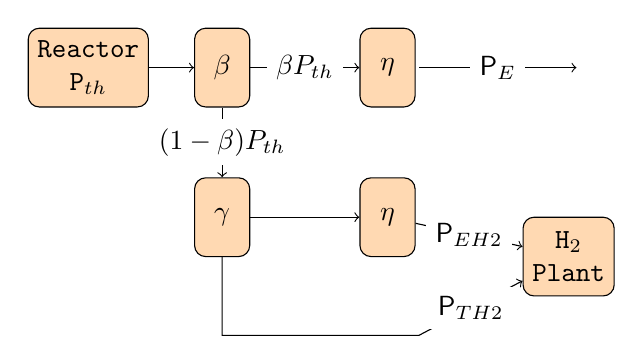
\begin{tikzpicture}[
    base/.style = {rectangle, rounded corners, draw=black,
minimum width=1.4cm, minimum height=1cm,
text centered, font=\sffamily},
process/.style = {base, minimum width=0.7cm, fill=orange!30,
font=\ttfamily},
node distance=1.4cm,
every node/.style={fill=white, font=\sffamily}, align=center
]

  \node (reactor) [process] {Reactor\\P$_{th}$};
  \node (div1) [process, right of=reactor, xshift=0.3cm] {$\beta$};
  \node (conv1) [process, right of=div1, xshift=0.7cm] {$\eta$};
  \node (div2) [process, below of=div1, yshift=-0.5cm] {$\gamma$};
  \node (conv2) [process, below of=conv1, yshift=-0.5cm] {$\eta$};
  \node (hydro) [process, right of=conv2, xshift=0.9cm, yshift=-0.5cm] {H$_2$\\Plant};

  \draw[->]     (reactor) -- (div1);
  \draw[->]     (div1) -- (conv1) node[midway] {$\beta P_{th}$};
  \draw[->]     (conv1) ++(0.4,0.)-- ++(2.0,0.) node[midway] {P$_E$};
  \draw[->]     (div1) -- (div2) node[midway] {$(1-\beta) P_{th}$};
  \draw[->]     (div2) -- (conv2);
  \draw[->]     (conv2) -- (hydro) node[midway] {P$_{EH2}$};
  \draw[->]     (div2) ++(0.,-0.5)-- ++(0.,-1.0)-- ++(2.5,0.) -- (hydro) node[midway] {P$_{TH2}$};

\end{tikzpicture}
}

\end{document}

% To compile do make; make -f hte1.makefile